\documentclass[aspectratio=169,11pt,usenames,dvipsnames]{beamer}

\usepackage[english]{babel}
\usepackage{graphicx}
\usepackage{enumitem}
\setlist[itemize,1]{label=\textbullet}
\setlist[itemize,2]{label=$\circ$}
\usepackage{amsmath}
\usepackage{mathtools}
\usepackage{float}
\usepackage{tikz}
\usetikzlibrary{patterns,arrows.meta}
\usepackage{tkz-euclide}
\tikzset{point style/.style = {%
  draw = black,
  inner sep = 0pt,
  shape = circle,
  minimum size = 5pt,
  fill = black
 }
}
\usepackage{booktabs} 
\usepackage{pgfplots}
\pgfplotsset{compat=1.18}
\usepackage{pgf-pie}

\usepackage{enumitem}

\usepackage{caption}
\usepackage{subcaption}

% Flowchart stuff

\usepackage{pgfopts}
\usepackage{xcolor}
\usepackage{tcolorbox}

\usetheme[
 titlestyle=style2,
 titleformat=smallcaps,
 sectionstyle=plain,
 slidestyle=cyber,
 headingcolor=theme,
 block=transparent
]{trigon}

\title{Probability}
\date{\today}
\author{Adam Klepáč}
\institute[GEVO]{Gymnázium Evolution Jižní Město}
\biglogo[width=.2\textwidth]{logo}
\smalllogo[width=.1\textwidth]{logo}
\titlegraphic{
\includegraphics[height=\paperheight]{title.jpg}}

\def\subsectionname{}

% enumerate global settings
\setlist[enumerate,1]{label=\arabic*.}
\setlist[enumerate,2]{label=\alph*)}

% custom colors %
\definecolor{DarkRed}{HTML}{260104}
\definecolor{LightRed}{HTML}{8C031C}
\definecolor{Red}{HTML}{590212}
\definecolor{Gray}{HTML}{4D4A59}
\definecolor{DarkBrown}{HTML}{0D0000}
\colorlet{tPrim}{DarkRed}
\colorlet{tTheme}{LightRed}
\colorlet{tSec}{LightRed}
\colorlet{tAccent}{Gray}
\colorlet{tText}{DarkBrown}

\newcommand{\clr}{\textcolor{BrickRed}}
\newcommand{\clb}{\textcolor{RoyalBlue}}
\newcommand{\clg}{\textcolor{ForestGreen}}
\newcommand{\clm}{\textcolor{Magenta}}

\tcbset{
 boxsep=7pt,
 fonttitle=\sc,
 colframe=tGreyBg,
 colframe=tTheme,
 boxrule=1pt
}

\begin{document}
\titleframe

\section{Probabilistic Intuition}
\label{sec:probabilistic-intuition}

\begin{frame}
 \frametitle{What Is Chance?}
 Imagine you have 9 balls of different colours.\pause
 \begin{center}
  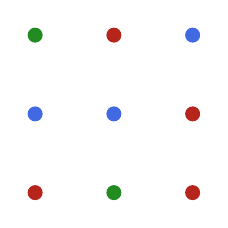
\begin{tikzpicture}
   \foreach \x in {0,1,2} {
    \foreach \y in {0,1,2} {
     \tkzDefPoint(\x,\y){\x\y}
    }
   }
   \tkzDrawPoints[color=BrickRed](00,12,20,21)
   \tkzDrawPoints[color=RoyalBlue](01,11,22)
   \tkzDrawPoints[color=ForestGreen](02,10)
  \end{tikzpicture}
 \end{center}
 \pause
 \begin{itemize}
  \item If you pick a ball \alert{at random}, what colour is it most likely to
   be?\pause
  \item How many times more likely is picking a \clr{red} ball than picking a
   \clg{green} ball?\pause
 \end{itemize}
\end{frame}

\begin{frame}
 \frametitle{Quantifying Probability}
 \begin{tcolorbox}[title=Probability]
  A \alert{probability} is a number between $0$ and $1$ measuring how
  \alert{likely} is something to happen.
 \end{tcolorbox}
\end{frame}

\begin{frame}
 \frametitle{Quantifying Probability -- Example}
 In our example of 9 balls
 \begin{center}
  \vspace*{-2em}
  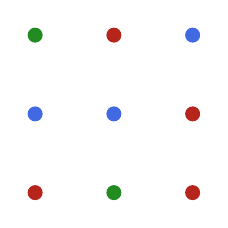
\begin{tikzpicture}
   \foreach \x in {0,1,2} {
    \foreach \y in {0,1,2} {
     \tkzDefPoint(\x,\y){\x\y}
    }
   }
   \tkzDrawPoints[color=BrickRed](00,12,20,21)
   \tkzDrawPoints[color=RoyalBlue](01,11,22)
   \tkzDrawPoints[color=ForestGreen](02,10)
  \end{tikzpicture}
 \end{center}
 what is the probability of picking a ball of a specific colour?\pause
 \begin{itemize}
  \item For \clr{red}, it's $4 / 9$.
  \item For \clb{blue}, it's $3 / 9$.
  \item For \clg{green}, it's $2 / 9$.
 \end{itemize}\pause
 The probabilities above \alert{sum up to $1$} because I am certain to pick
 \emph{some} ball.
\end{frame}

\begin{frame}
 \frametitle{Quantifying Probability -- Example}
 We'll all the outcome of a random choice, a \alert{random variable} and
 typically write it as $X$.\pause\\
 A random variable always lies in the set of all possible outcomes.\pause\\
 In this case, the variable $X$ must lie in the set of possible colours,
 $\{\clr{\text{red}},\clb{\text{blue}},\clg{\text{green}}\}$.\pause\\
 We'll write the probability that $X$ is equal to one of the elements in the set
 as $P(X=\text{colour})$.\pause\\
 So, for the 9-ball example from before, we would have
 \[
  P(X=\text{\clr{red}}) = \frac{4}{9}, \quad P(X=\text{\clb{blue}}) =
  \frac{3}{9}, \quad P(X=\text{\clg{green}}) = \frac{2}{9}.
 \]
\end{frame}

\begin{frame}
 \frametitle{Calculating Probability}
 In the case the set of outcomes is \alert{finite}, the probability of $X$ being
 one of the possible outcomes is always\pause
 \begin{tcolorbox}
  \[
   P(X \in S) = \frac{|S|}{|O|},
  \]
 \end{tcolorbox}
  where $S$ is a certain subset of $O$ -- all the possible outcomes.
\end{frame}

\begin{frame}
 \frametitle{Calculating Probability -- Example}
 We'll describe our 9-ball example more formally.\pause\\
 We'll assign the balls number from $1$ to $9$. The set of all possible outcomes
 of picking a random ball is then
 \[
  O = \{1,2,3,4,5,6,7,8,9\}.
 \]
 \begin{center}
  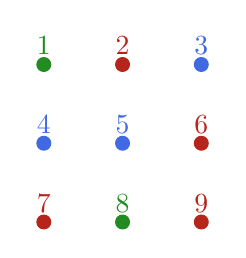
\begin{tikzpicture}
   \foreach \x in {0,1,2} {
    \foreach \y in {0,1,2} {
     \tkzDefPoint(\x,\y){\x\y}
    }
   }
   \tkzDrawPoints[color=BrickRed](00,12,20,21)
   \tkzDrawPoints[color=RoyalBlue](01,11,22)
   \tkzDrawPoints[color=ForestGreen](02,10)

   \tkzLabelPoint[above,color=BrickRed](00){$7$}
   \tkzLabelPoint[above,color=BrickRed](12){$2$}
   \tkzLabelPoint[above,color=BrickRed](20){$9$}
   \tkzLabelPoint[above,color=BrickRed](21){$6$}

   \tkzLabelPoint[above,color=RoyalBlue](01){$4$}
   \tkzLabelPoint[above,color=RoyalBlue](11){$5$}
   \tkzLabelPoint[above,color=RoyalBlue](22){$3$}

   \tkzLabelPoint[above,color=ForestGreen](02){$1$}
   \tkzLabelPoint[above,color=ForestGreen](10){$8$}
  \end{tikzpicture}
 \end{center}
\end{frame}

\begin{frame}
 \frametitle{Calculating Probability -- Example}
 \begin{center}
  \vspace*{-1em}
  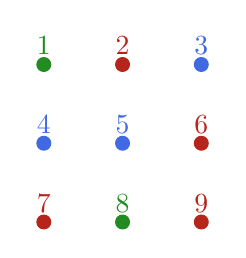
\begin{tikzpicture}
   \foreach \x in {0,1,2} {
    \foreach \y in {0,1,2} {
     \tkzDefPoint(\x,\y){\x\y}
    }
   }
   \tkzDrawPoints[color=BrickRed](00,12,20,21)
   \tkzDrawPoints[color=RoyalBlue](01,11,22)
   \tkzDrawPoints[color=ForestGreen](02,10)

   \tkzLabelPoint[above,color=BrickRed](00){$7$}
   \tkzLabelPoint[above,color=BrickRed](12){$2$}
   \tkzLabelPoint[above,color=BrickRed](20){$9$}
   \tkzLabelPoint[above,color=BrickRed](21){$6$}

   \tkzLabelPoint[above,color=RoyalBlue](01){$4$}
   \tkzLabelPoint[above,color=RoyalBlue](11){$5$}
   \tkzLabelPoint[above,color=RoyalBlue](22){$3$}

   \tkzLabelPoint[above,color=ForestGreen](02){$1$}
   \tkzLabelPoint[above,color=ForestGreen](10){$8$}
  \end{tikzpicture}
  \vspace*{-1em}
 \end{center}
 We'll form three subsets of $O$:
 \begin{align*}
  \clr{R} &= \{\clr{2},\clr{6},\clr{7},\clr{9}\},\\
  \clb{B} &= \{\clb{3},\clb{4},\clb{5}\},\\
  \clg{G} &= \{\clg{1},\clg{8}\}.
 \end{align*}\pause
 We can use the formula from before to calculate the probability that $X$ will
 be a \clg{green} ball:
 \[
  P(X \in \clg{G}) = \frac{|\clg{G}|}{|O|} = \frac{2}{9}.
 \]
\end{frame}

\section{Probability Equations}
\label{sec:probability-equations}

\begin{frame}
 \frametitle{Sums of Probabilities}
 What if I asked about the probability that the ball I pick is \clr{red} or
 \clb{blue}?\pause\\
 We can literally use the same formula as before. Now, the set of outcomes we're
 interested in is $\clr{R} \cup \clb{B}$ and so\pause
 \[
  P(X \in \clr{R} \cup \clb{B}) = \frac{|\clr{R} \cup \clb{B}|}{|O|} =
  \frac{|\clr{R}| + |\clb{B}|}{|O|} = \frac{4+3}{9} = \frac{7}{9}.
 \]
 \pause
 However, this example cannot be easily generalized. We'll see why.
\end{frame}

\begin{frame}
 \frametitle{Sums of Probabilities -- Counterexample}
 Suppose we're instead choosing from a set of numbers between $1$ and
 $20$.\pause\\
 We want to calculate the probability that a randomly picked number is
 \alert{even or divisible by $5$}.\pause\\
 So, we have
 \begin{align*}
  O &= \{1,2,\ldots,20\},\\
  E &= \{2,4,6,\ldots,20\},\\
  F &= \{5,10,15,20\}.
 \end{align*}\pause
 and we want to figure out the probability $P(X \in E \cup F)$.
\end{frame}

\begin{frame}
 \frametitle{Sums of Probabilities -- Counterexample}
 Let's try to use the same formula as before:
 \[
  P(X \in E \cup F) = \frac{|E \cup F|}{|O|} \overset{??}{=} \frac{|E| +
  |F|}{|O|} = \frac{10 + 4}{20} = \frac{14}{20}.
 \]\pause
 This doesn't quite add up.\pause\\
 If we count such numbers by hand, we get the set
 \[
  \{2,4,5,6,8,10,12,14,15,16,18,20\}.
 \]
 \pause
 There's \alert{only 12 of them}.\pause\\
 The problem is that \alert{we counted the numbers 10 and 20 twice}!\pause\\
 So, to get the size of $E \cup F$, we cannot just add the size of $E$ to the
 size of $F$ but we also have to subtract the elements that appear twice -- the
 size of $E \cap F$.
\end{frame}

\begin{frame}
 \frametitle{Sums of Probabilities -- Formula}
 The previous example applies in general. If $A,B$ are two subsets of the set of
 outcomes, $O$, then\pause
 \begin{tcolorbox}
  \[
   P(X \in A \cup B) = \frac{|A \cup B|}{|O|} = \frac{|A| + |B| - |A \cap
   B|}{|O|}.
  \]
 \end{tcolorbox}
\end{frame}

\end{document}
